%!TEX root = ../main.tex
\section{Joint Board Software Development} % (fold)
\label{sub:joint_board_software}

\subsection{Analysis} % (fold)
\label{ssub:joint_board_analysis}
The main responsibility of the joint software is to maintain knowledge of the angle of its joint and transmit that angle to the controller board.
The following analysis will elaborate on the needed functionalities and requirements for the software.

\subsubsection{Joint Angle}
The angle of the joint can be determined by analysing the signals from the RL2IC encoder mounted on the joint.

This encoder implements incremental quadrature with three signals: \texttt{A}, \texttt{B} and \texttt{Z}.
Figure \ref{fig:quadrature} is a depiction of this quadrature scheme.
The two signals \texttt{A} and \texttt{B} are 90$^\circ$ out of phase and their frequency is determined by the angular velocity of the joint.
As can be seen from the figure the signals create four unique stages, counting these allows knowledge of both the direction, position and, potentially, the velocity of the joint.

\begin{figure}[h]
	\centering
	
\includegraphics[width=.5\linewidth]{graphics/quadrature}
	\caption[Incremental quadrature scheme RL2IC encoder.]{Incremental quadrature scheme as implemented on the RL2IC encoder.}
	\label{fig:quadrature}
\end{figure}

It is necessary to read \texttt{A}, \texttt{B} and \texttt{Z} using interrupts as missing a cycle or introducing jitter in the counting procedure will cause the measured angle to drift.
\texttt{Z} only goes \texttt{high} one time per revolution and can therefore be used to infer the absolute angle of the joint.
This should be done by calibrating the joint angle by setting  the measured angle to a fixed number, whenever \texttt{Z} goes \texttt{high}.
This means that the angle should not be measured until the joint software has been calibrated by reaching the point where \texttt{Z} goes \texttt{high}.

Since the angle is to be transmitted there is a risk that an interrupt may occur while this transmission takes place, potentially corrupting the data to be transmitted.
This needs to be avoided and can be done by temporarily disabling interrupts and copying the needed data to other variables.
The code that temporarily disables interrupts and copies the variable needs to be executed faster than two consecutive interrupts can occur, because otherwise angle movement is lost.
The time between two consecutive interrupts is only dependent of the angular velocity of the joint.
It is estimated that the maximum angular velocity is  $\approx$20Hz, which means that no interrupts should go unnoticed at this frequency.
\mikkel{It would be nice with some sort of reasoning/reference.}

\subsubsection{Wireless Transmission of Data}
As mentioned in section \ref{ssub:interboard_communication}, communication between the controller board and the joint boards is to happen wirelessly using the \texttt{nRF24L01} module and a period between packets of more than 130$\mu$s.
The software needs to communicate with the \texttt{nRF24L01} through a SPI connection with the \texttt{ATtiny} as the master.
The \texttt{nRF24L01} has a number of options that needs to be set according to the wanted functionality.
As described in \ref{ssub:interboard_communication}, it was found that the two joints needs to send using two separate frequency bands to avoid air collisions. 
This needs to be set up individually in each \texttt{nRF24L01} module. 
Latency should be minimized by reducing overhead in transmitted packages and sending the smallest possible payload that correctly conveys the joint data.
The data sheet describes that the \texttt{nRF24L01} can operate at air rates of 250kbps, 1Mbps and 2Mbpthat.
The transmission tests in \ref{} ....
a transmission rate of 1Mbps was chosen.. 

\paragraph{Transmission Rate} % (fold)
\label{par:transmission_rate}~\\
The datasheet of the \texttt{nRF24L01} module specifies that there is a settling time of 130$\mu$s when entering the transmit state.
Several aspects should be considered in order to determine the required period time associated with transmission of one data packet. 
Transmission of a two byte payload through SPI takes $\approx$ 36 $\mu$s as will be shown in \ref{}.
The \texttt{CE} should be high for at least 10$\mu$s in order for the transition to transmit mode is initiated.
Hereafter the settling time of 130$\mu$s is inferred.
Then the \texttt{nRF24L01} will transmit the two byte payload in a eight byte data packet, which will take 68$\mu$s using a air transmission rate of 1Mbps.
This totals 244$\mu$s, in which the computation time needed is not included.
Therefore it was decided to use a period time of 333$\mu$s, which yields 89$\mu$s to computation and a sampling frequency of $\approx$3kHz.
The period is shown in figure \ref{fig:tiny_period}.

\begin{figure}[h]
	\centering
	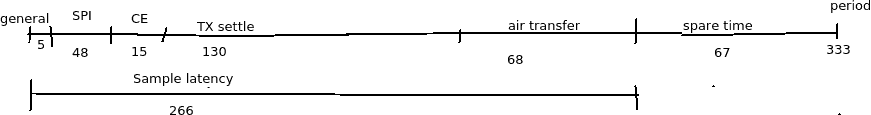
\includegraphics[width=1\linewidth]{graphics/tiny_period}
	\caption[Period of wireless transmission]{Period associated with transmission of one data packet.}
	\label{fig:tiny_period}
\end{figure}



\subsubsection{Real Time Software}
In order to produce reliable data for the controller board the joint angle should be sampled and transmitted at a constant rate.
This requires the joint board software to be programmed as real time software, where deadlines should be met.

\subsection{Requirement Specification} 

\paragraph{Functional:}
\begin{enumerate}[resume]
	\item Correct joint angle should be known at all times.
	\label{enum:joint_correct_angles}
	\begin{enumerate}
		\item Encoder signals \texttt{A}, \texttt{B} and \texttt{Z} should be interfaced using interrupts.
		\item \texttt{A}, \texttt{B} should be used to measure the relative angle.
		\item \texttt{Z} should be used to infer the absolute angle. 
		\item Determine movement and direction of movement based on encoder signals.
		\item Ensure no data is corrupted by interrupts.
		\item Ensure no interrupts lost at angular frequencies below 20Hz.
	\end{enumerate}
	\item Transmit joint angle using the \texttt{nRF24L01} module.
	\label{enum:joint_transmit}
	\begin{itemize}
		\item Setup of the \texttt{ATtiny} as a SPI master.
		\item Setup of \texttt{nRF24L01} settings and individually frequency bands.
		\item Transmit data every 333$\mu$s.
		\item Minimize latency.
	\end{itemize}
	\item Real time behaviour of software.
	\label{enum:joint_real_time}
\end{enumerate}

\subsection{Design and Implementation} % (fold)
\label{sub:design_and_implementation}

\mikkel{Add attiny84 setup before nrf setup. Add calibrated = 1.}
\begin{figure}[h]
	\centering
	\begin{subfigure}[b]{0.30\textwidth}
		\centering
		\includegraphics[width=.8\linewidth]{graphics/joint_software_diagram}
		\caption{Main loop.}
		\label{sfig:joint_main_flowchart}
	\end{subfigure}
	\begin{subfigure}[b]{0.69\textwidth}
		\centering
		\includegraphics[width=.8\linewidth]{graphics/joint_interrupt}
		\caption{Encoder signal Interrupt Service Routine.}
		\label{sfig:joint_interrupt}
	\end{subfigure}
	\caption{Flowchart of the software design for the joint board.}
	\label{fig:joint_software}
\end{figure}
A software design was made based on the requirements for the joint board software.
The main functionality of the software is illustrated in the flowchart of figure \ref{sfig:joint_main_flowchart}.
Upon startup the \texttt{nRF24L01} is setup as explained in section \ref{par:nrf24l01}.
A timer is initiated to ensure that a packet, as shown in figure \ref{fig:rfpacket}, is sent every 333$\mu$s.
Now the copying procedure is started after which the packet is transmitted and the program is idling until 333$\mu$s has passed and the process starts over.
An interrupt can happen at any given time and the ISR, will update the measured joint angle. 
The coming sections will elaborate on the different elements of the software.

\subsubsection{Joint Angle Measurement}
\label{ssub:joint_angle_measurement}
In figure \ref{sfig:joint_interrupt} the interrupt routine is shown.
This routine can be engaged at any given time and is engaged whenever an either rising or falling edge appears on \texttt{A}, \texttt{B} or \texttt{Z}.

Initially the signals are read.
If \texttt{Z} is high the index has been reached and the position counter is reset and the calibration bit is set.
Hereafter the execution of the main loop is continued.
If \texttt{Z} is low \texttt{A} and \texttt{B} are inspected to determine which phase is active.
Table \ref{tab:bin_phase} shows each phase and the combination of \texttt{A} and \texttt{B} in that phase.
By comparing with the previous phase it is possible to determine the direction of movement and therefore whether the position counter should be incremented or decremented.
Before returning execution to the main loop the current phase is stored. 

\begin{table}
	\centering
	\begin{tabular}{c | c  c}
		& \texttt{A} & \texttt{B}\\
		\hline
		P1 & 0 & 1\\
		P2 & 0 & 0\\
		P3 & 1 & 0\\
		P4 & 1 & 1
	\end{tabular}
	\caption{Binary representation of the phases.}
	\label{tab:bin_phase}
\end{table}

\subsubsection{Wireless Transmission of Data}
\label{ssub:wireless_transmission_of_data}
The joint board should transmit the angular angle of the joint and whether calibration has occured since startup.
The \texttt{RL2IC} encoder used in the joint produces 7200 counts per revolution, requiring 13 bits to represent a full revolution of the joint.
The calibration status is binary and represents one bit. 
16 bit is required to transmit this information, since the \texttt{nRF24L01} payload needs be an integer number of bytes.
See figure \ref{fig:rfpacket} for a visual representation of the message.

\mikkel{Joint ID, calibration and direction not necessary }
\begin{figure}[h]
	\centering
	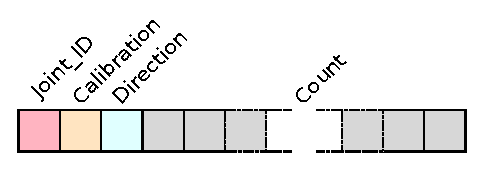
\includegraphics[width=.5\linewidth]{graphics/rf_packet}
	\caption[RF transmission packet used from the joint board.]{UPDATE ME!!!!!!!!!!!!!!--  Sructure of a packet used on the RF transmission between the joint boards and the controller board. Bits 0-12 represent the current joint angle and bit 13 represents the state of calibration.}
	\label{fig:rfpacket}
\end{figure}

When information is to be transmitted the calibration and angle variables needs to be copied to other variables.
The act of copying a variable takes several clock cycles and if an interrupt occurs while the variable is being transmitted the data is can be corrupted.
In order to avoid this problem it is necessary to temporarily disable interrupts while copying original variable into a temporary variable. 
In effect the resulting code is as seen in code \ref{code:critical_section_c}.
Disabling interrupts means that any incoming interrupts will not be processed until interrupts are reenabled, as described in the datasheet of the ATtiny84 \cite{attiny84}.
Interrupts should therefore not be disabled for longer than the shortest expected time between two edges on any single signal.

The \texttt{AVR-GCC} compiler has the option to only compile the code, leaving a human readable assembly file.
The assembly corresponding to code \ref{code:critical_section_c} can be seen in code \ref{code:critical_section_asm}.
Each of these instructions are described in the datasheet of the microcontroller where the number of cycles required to execute them is specified: \texttt{rcall} 3 cycles, \texttt{\_CLI} 1 cycle, \texttt{ldd} 2 cycles, \texttt{std} 2 cycles, \texttt{\_SEI}, 1 cycle.
In total 16 clock cycles are spent executing the required commands.
At 8MHz this is 2 $\mu$s.
Since the RL2IC produces 7200 ticks per revolution only 3600 edges exist on a single signal per revolution. 
Using these numbers the theoretical maximum angular velocity possible while still maintaining more than 2 $\mu$s between each edge on a signal is $\approx$135Hz, which is clearly above the estimated maximum velocity of $\approx$20Hz.

\begin{listing}[h] 
\begin{minted}{c}
	_CLI();
	cnt_temp=cnt;
	_SEI();
\end{minted}
\caption{Critical section for copying counter value. C version.}
\label{code:critical_section_c}
\end{listing}

{\renewcommand\fcolorbox[4][]{\textcolor{cyan}{\strut#4}}
\begin{listing}[h]
\begin{minted}{gas}
	rcall _CLI
	ldd r24,Y+1
	ldd r25,Y+2
	std Y+4,r25
	std Y+3,r24
	rcall _SEI
\end{minted}
\caption{Critical section for copying counter value. Assembly version.}
\label{code:critical_section_asm}
\end{listing}


\subsubsection{SPI} % (fold)
\label{ssub:spi}
The \texttt{ATtiny84} does not have a SPI controller, but it does have a Universal Serial Interface, USI, which is compatible with SPI, when it is used in its three wire mode.
In this mode the interface has the pins, Data Out \texttt{DO}, Data In \texttt{DI} and a clock \texttt{USCK}.
In order to comply with the SPI standard a Slave Select \texttt{SS} pin should be implemented using a general IO pin and custom written software.
The \texttt{nRF24L01} also has a non SPI pin, \texttt{CE} that also needs to be controlled from the \texttt{ATtiny}.
The full interface between the two is shown in figure \ref{fig:tiny_nrf_com}.

\begin{figure}[h]
	\centering
	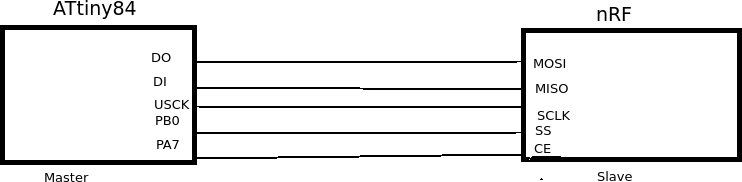
\includegraphics[width=.8\linewidth]{graphics/tiny_nrf_com}
	\caption[Interface between ATtiny84 and nRF24L01.]{Interfacing the \texttt{ATtiny84}s USI and \texttt{nRF24L01}s SPI. \texttt{PB0} and \texttt{PA7} are general purpose IO pins.}
	\label{fig:tiny_nrf_com}
\end{figure}
The \texttt{ATtiny84} is used as the SPI master and controls \texttt{MOSI}, \texttt{SCLK}, \texttt{SS} and \texttt{CE} on the \texttt{nRF24L01} module.

With the two modules interfaced correctly, data can be transmitted between them.
The function shown in listing \ref{code:tiny_spi_transfer} implements this functionality on the \texttt{ATtiny84}.
It takes pointers to \texttt{data}, \texttt{input} and the number of bytes that needs to be sent as inputs.
Line 2 sets \texttt{SS} \texttt{low} to initiate an SPI transfer.
The loop in lines 4 to 11 is run \texttt{n} times to send and receive \texttt{n} bytes.
In line 5 the USI Data Register \texttt{USIDR} is loaded with the byte to be sent and in line 6 the counter overflow flag in the USI Status Register, \texttt{USISR}, is cleared.
Lines 7 to 9 writes 1 to the \texttt{USITC} bit of the USI Control Register \texttt{USICR} until the counter overflow flag \texttt{USIOIF} is raised.
The USI clock \texttt{USCK} is toggled each time 1 is written to \texttt{USITC}.
Data is shifted to \texttt{DO} correctly by the USI by counting the clock edges generated. 
Data on \texttt{DI} is sampled at falling edges of the \texttt{USCK} and stored in \texttt{USIDR}.
The counter overflow flag \texttt{USIOIF} will raise when 16 clock edges has been generated and eight bits of data has been sent and received.
Line 10 copies the received data to the \texttt{input} pointer if there is one.
When \texttt{n} bytes of data has been sent and received the \texttt{SS} pin will be set \texttt{high} and the function is exited.
\mikkel{Does this shit make sense or do we need to add some other kind of illustration or explanation.}
\begin{listing}[h] 
\begin{minted}{c}
void spi_transfer(uint8_t *data, uint8_t *input, uint8_t n){
  PORTB &= ~_BV(SS);
  int i;
  for(i = 0; i<n; i++){
	USIDR = data[i];
	USISR = _BV(USIOIF);  
	while ( !(USISR & _BV(USIOIF)) ){
		USICR |= _BV(USITC);  
	} 
	if(NULL |= input){input[i] = USIDR;}
  }
  PORTB |= _BV(SS);
}
\end{minted}
\caption{Function that transmits \texttt{n} bytes of data between the \texttt{ATtiny84} and the \texttt{nRF24L01}.}
\label{code:tiny_spi_transfer}
\end{listing}

This functions enables setup of the \texttt{nRF24L01}, which is done with the same settings as explained in section \ref{ssubs:nrf24l01}.


\subsubsection{Software Timer}
\label{ssub:software_timer}
The timer shown in figure \ref{sfig:joint_main_flowchart}, is implemented on the \texttt{ATtiny84} using \texttt{Counter 1}, which is a 16 bit timer capable of generating software interrupts.
\texttt{Counter 1} is setup by setting a prescaler to the CPU clock and a compare value.
Using a prescaler of 1, the compare value for setting up a interrupt each 333$\mu$s is calculated as: 
\begin{equation}
	Comp = \frac{T}{T_{cpu}} = \frac{333 \cdot 10^{-6}}{1.25\cdot 10^{-7}} = 2664
\end{equation}
Where $Comp$ is the compare value, $T$ is the wanted period time and $T_{cpu}$ is the cpu clock period.
Setting up \texttt{Counter 1} with this compare value and the flag to clear the counter when reaching the compare value, results in interrupts on \texttt{TIM1\_COMPA\_vect} each 333$\mu$s.

\begin{listing}[h] 
\begin{minted}{c}
volatile char timer;

ISR(TIM1_COMPA_vect)
{ 
  timer = 1;
}
\end{minted}
\caption{Counter \texttt{ISR} function and declaration of \texttt{timer}.}
\label{code:timer_isr}
\end{listing}

The ISR function associated with these interrupts are shown in \ref{code:timer_isr} together with the declaration of \texttt{timer}.
The variable is declared as \texttt{volatile} to tell the compiler that its value is changed in an \texttt{ISR}. 
It is declared as a \texttt{char}, because this is the smallest datatype available on the \texttt{ATtiny84} and it only takes up one byte. 
In the main loop of the software, the \texttt{timer} variable is used determine if the process of transmitting data should be initiated.
This mechanism provides real time performance of the software when the code used to transmit data is executed before the next deadline, which is the next \texttt{counter 1} interrupt.
This means that the transmitting code needs to be executed in less than 333$\mu$s to ensure real time performance.

\begin{listing}[h] 
\begin{minted}{c}
while(1){
    if(timer==1){ 
      	timer = 0;
      		@$\vdots$@
      	// Transmit data
			@$\vdots$@      
	}
}
\end{minted}
\caption{Main loop of the software. The \texttt{timer} variable is used to transmit data at a fixed frequency.} 
\label{code:main_loop_timer}
\end{listing}
In lines 2 and 3 of listing \ref{code:main_loop_timer} the \texttt{timer} variable is accessed.  
Accessing a variable that is written to in a \texttt{ISR} can result in corrupted data, but in this case it is not a problem because \texttt{timer} is a one byte variable. 
The two assembly instructions that will be used to access the value of \texttt{timer} is \texttt{ldi} and \texttt{cpi}, which are both instructions that will be executed in one clock cycle.

\subsection{Verification} % (fold)
\label{sub:verification}


\subsubsection{Requirement \ref{enum:joint_correct_angles}} % (fold)
\label{ssub:requirement_enum:correct_angles}
Requirement \ref{enum:joint_correct_angles} specifies that the correct joint angle should be know at all times.
This cannot be verified without utilizing the wireless transmission between the joint board and controller as the only other output the jointboard has is a LED.

\texttt{A}, \texttt{B} and \texttt{Z} signals were interfaced through interrupts and the code was written to ensure no data will be corrupted by interrupts.
Calculations showed that no interrupts will go unnotieced with a angular velocity of less than 135Hz. 

\paragraph{Test}~\\
A test was conducted where the joint angle information was sent to the controllerboard and printed to a serial console. 
By visual inspection the functionality was verified.

\subsubsection{Requirement \ref{enum:joint_transmit} and \ref{enum:joint_real_time}} % (fold)
\label{ssub:requirement_enum:joint_transmit}

\paragraph{Test}~\\

\paragraph{Result}~\\